%%%%%%%%%%%%%%%%%%%%%%%%%%%%%%%%%%%%%

\section{1.4.Estudos observacionais e métodos de amostragem}

%%%%%%%%%%%%%%%%%%%%%%%%%%%%%%%%%%%%

\subsection{Confundindo}

%%%%%%%%%%%%%%%%%%%%%%%%%%%%%%%%%%%%

\begin{frame}
\frametitle{}

\begin{center}
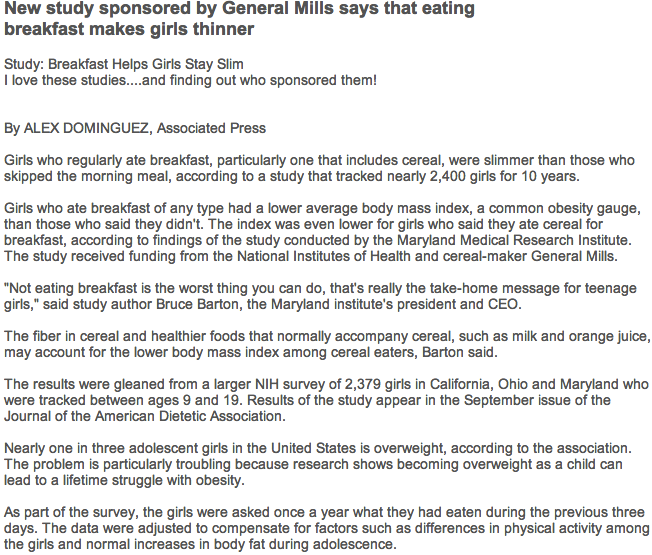
\includegraphics[width=0.80\textwidth]{1-4_obs_studies_sampling/figures/breakfast/breakfast1.png}
\end{center}

{\tiny \webURL{http://www.peertrainer.com/LoungeCommunityThread.aspx?ForumID=1\&ThreadID=3118}}

\end{frame}
%%%%%%%%%%%%%%%%%%%%%%%%%%%%%%%%%%%%

\begin{frame}
\frametitle{Tradução Texto}
\justifying
\tiny{
Novo estudo patrocinado pela General Mills diz que tomar o café da manhã deixa as meninas mais magras.\\
\vspace{0.2 cm}
Estudo: Café da manhã ajuda as meninas a permanecerem magras\\
\vspace{0.2 cm}
Eu amo esses estudos ... e descobrir quem os patrocinou!\\
\vspace{0.2 cm}
Por ALEX DOMINGUEZ, Jornalista associado.\\
\vspace{0.5 cm}
Garotas que tomam café da manhã regularmente, especialmente uma que inclui cereal, são mais magras do que as que pularam a refeição da manhã, de acordo com um estudo que acompanhou quase 2.400 garotas por 10 anos.\\

Meninas que tomavam o café da manhã de qualquer tipo tinham um índice de massa corporal médio menor, um índice de obesidade comum, daquelas que diziam que não o faziam. O índice foi ainda menor para as meninas que disseram que comeram cereais no café da manhã, de acordo com as conclusões do estudo realizado pelo Instituto de Pesquisa Médica de Maryland. O estudo recebeu financiamento do Instituto Nacional de Saúde e da fabricante de cereais General Mills.\\

"Não comer o café da manhã é a pior coisa que você pode fazer, é realmente a mensagem para as adolescentes", disse o autor do estudo, Bruce Barton, presidente e CEO do Instituto Maryland.\\

A fibra nos cereais e alimentos mais saudáveis que normalmente acompanham o cereal, como leite e suco de laranja, podem ser responsáveis pelo menor índice de massa corporal entre os consumidores de cereais, disse Barton.\\

Os resultados foram obtidos a partir de uma pesquisa maior do NIH com 2.379 meninas na Califórnia, Ohio e Maryland, que foram rastreadas entre as idades de 9 e 19 anos. Os resultados dos estudos aparecem na edição de setembro do Jornal da Associação Dietética Americana.\\

Quase uma em cada três adolescentes nos Estados Unidos têm sobrepeso, segundo a associação. O problema é particularmente preocupante porque a pesquisa mostra que o excesso de peso de uma criança pode levar a uma luta pela obesidade.\\

Como parte da pesquisa, as garotas foram perguntadas uma vez por ano o que haviam comido durante os três dias anteriores.\\

Os dados foram ajustados para compensar fatores como diferenças na atividade física entre as garotas e aumentos normais na gordura corporal durante a adolescência.
}

\end{frame}
%%%%%%%%%%%%%%%%%%%%%%%%%%%%%%%%%%%%

\begin{frame}
\frametitle{}
\justifying
\dq{Que tipo de estudo é este, estudo observacional ou um experimental?}\\
{\footnotesize \textit{``Garotas que tomam café da manhã regularmente, especialmente um que inclui cereal, são mais magras do que as que pularam a refeição, de acordo com o estudo que acompanhou quase 2.400 garotas por 10 anos.[...] Como parte da pesquisa, uma vez por ano as garotas respondiam um questionário sobre o que haviam comido durante os três dias anteriores."}}


\soln{\onslide<2->{Isto é um \hl{estudo observacional} já que os pesquisadores apenas observaram o comportamento das meninas (sujeitos) em oposição à imposição de tratamentos sobre elas.}}

\dq{Qual é a conclusão do estudo??}

\soln{\onslide<3->{Há uma \hl{associação} entre garotas serem magras e tomarem café da manhã.}}

\dq{Quem patrocinou o estudo?}

\soln{\onslide<4->{Todas}}

\end{frame}

%%%%%%%%%%%%%%%%%%%%%%%%%%%%%%%%%%%%

\begin{frame}[shrink]
\frametitle{3 explicações possíveis}

\pause

\begin{enumerate}

\item Comer o café da manhã faz com que as meninas fiquem mais magras.
\begin{center}

\includegraphics[width=0.5\textwidth]{1-4_obs_studies_sampling/figures/breakfast/breakfast2.png}
\end{center}

\pause

\item Ser magra faz com que as meninas tomem café da manhã.
\begin{center}

\includegraphics[width=0.5\textwidth]{1-4_obs_studies_sampling/figures/breakfast/breakfast3.png}
\end{center}

\pause
\justifying
\item Uma terceira variável é responsável por ambas. O que poderia ser? \\
Uma variável estranha que afeta tanto a variável explicativa quanto a variável de resposta e que faz parecer que existe uma relação entre as duas.
\begin{center}
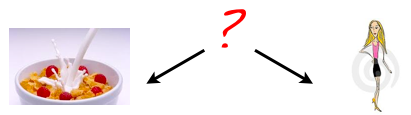
\includegraphics[width=0.5\textwidth]{1-4_obs_studies_sampling/figures/breakfast/breakfast4.png}
\end{center}

\end{enumerate}


{\tiny Images from: \webURL{http://www.appforhealth.com/wp-content/uploads/2011/08/ipn-cerealfrijo-300x135.jpg},  \webURL{http://www.dreamstime.com/stock-photography-too-thin-woman-anorexia-model-image2814892}.}



\end{frame}

%%%%%%%%%%%%%%%%%%%%%%%%%%%%%%%%%%%%

\begin{frame}
\frametitle{Estudos prospectivos vs. retrospectivos}

\begin{itemize}
\justifying
\item O estudo \hl{prospectivo} identifica indivíduos e coleta informações à medida que os eventos se desdobram.
\begin{itemize}
\justifying
\item Exemplo: Desde 1976 o Nurses Health Study (Estudo de Saúde para Enfermeiros nos EUA) tem recrutado enfermeiros e em seguida coletado dados por meio de questionários.
\end{itemize}
\justifying
\item \hl{Estudos retrospectivos} coletar dados após os eventos terem ocorrido.
\begin{itemize}
\justifying
\item Exemplo: Pesquisadores revisando eventos passados em registros médicos.
\end{itemize}

\end{itemize}

\end{frame}

%%%%%%%%%%%%%%%%%%%%%%%%%%%%%%%%%%%

\subsection{Métodos de amostragem}

%%%%%%%%%%%%%%%%%%%%%%%%%%%%%%%%%%%

\begin{frame}
\frametitle{Obtendo boas amostras}

\begin{itemize}
\justifying
\item Quase todos os métodos estatísticos são baseados na noção de aleatoriedade implícita.
\justifying
\item Se os dados observacionais não são coletados em uma estrutura aleatória, esses métodos estatísticos -- as estimativas e erros associados às estimativas -- não são confiáveis.
\justifying
\item As técnicas de amostragem aleatória mais comumente usadas são amostragem \hl{aleatória simples}, \hl{estratificado}, \hl{por conglomerados} e \hl{estratificada}.

\end{itemize}

\end{frame}

%%%%%%%%%%%%%%%%%%%%%%%%%%%%%%%%%%%%

\begin{frame}
\frametitle{Amostra aleatória simples}
\justifying
Seleciona aleatoriamente casos da população, onde não há conexão implícita entre os pontos selecionados.

\begin{center}
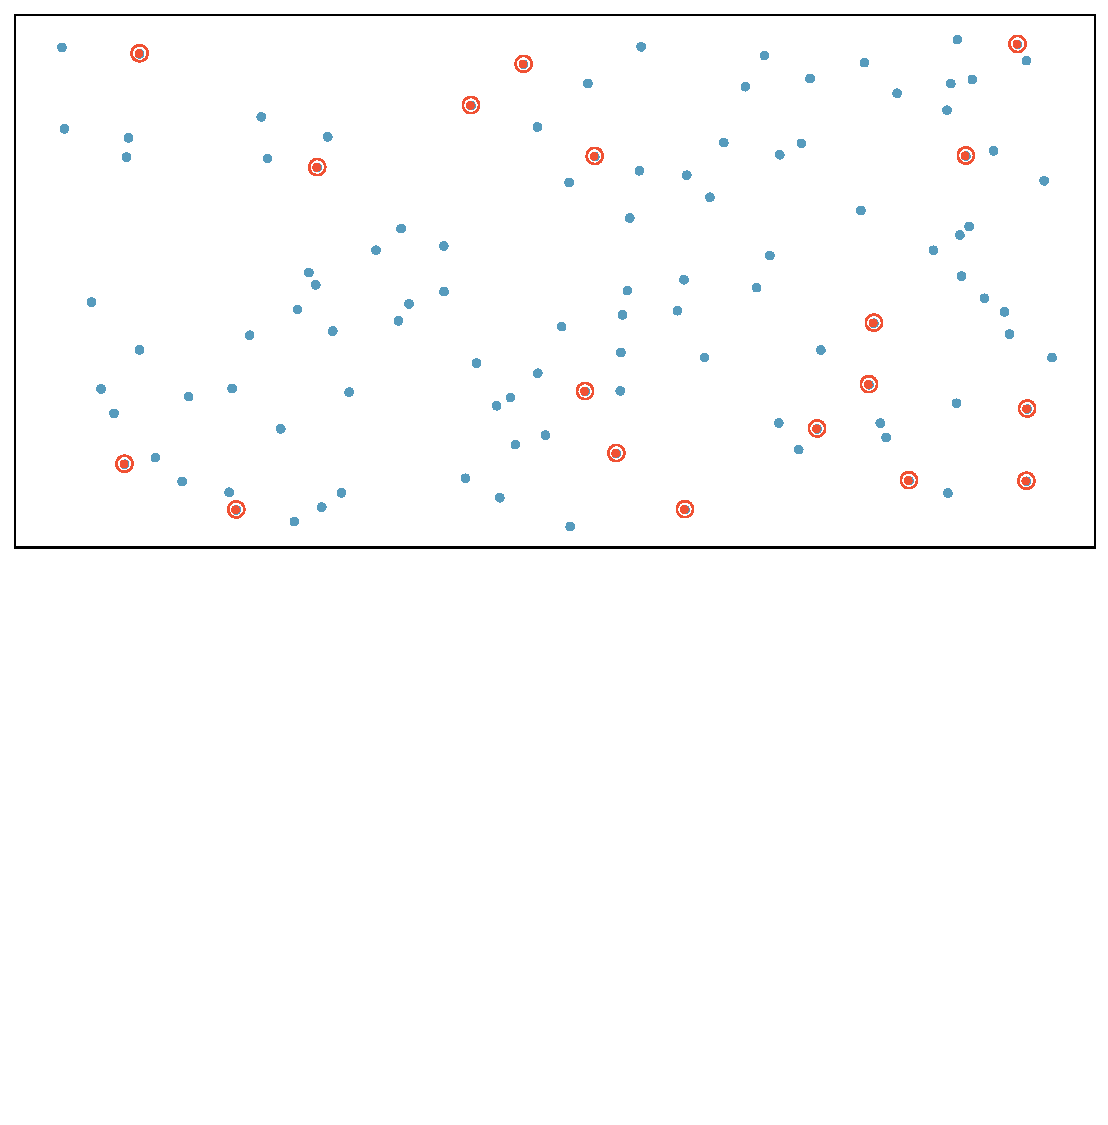
\includegraphics[width=0.9\textwidth]{1-4_obs_studies_sampling/simple.pdf}
\end{center}

\end{frame}

%%%%%%%%%%%%%%%%%%%%%%%%%%%%%%%%%%%%

\begin{frame}
\frametitle{Amostragem estratificada}
\justifying
\hl{Estratos} são constituídos por observações semelhantes. Seleciona-se uma amostra aleatória simples de \underline{cada} estrato.

\begin{center}
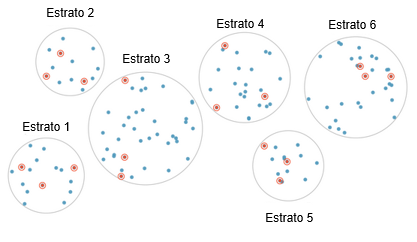
\includegraphics[width=0.9\textwidth]{1-4_obs_studies_sampling/stratified.png}
\end{center}

\end{frame}

%%%%%%%%%%%%%%%%%%%%%%%%%%%%%%%%%%%%

\begin{frame}
\frametitle{Amostragem por conglomerados}
\justifying
\hl{Grupos} geralmente não são feitos de observações homogêneas. Seleciona-se uma amostra aleatória simples dos conglomerados e, em seguida, \underline{todas} as observações nesse grupo. 

\begin{center}
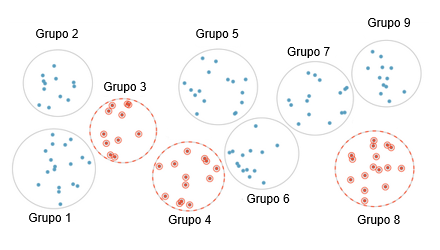
\includegraphics[width=0.9\textwidth]{1-4_obs_studies_sampling/cluster.png}
\end{center}

\end{frame}

%%%%%%%%%%%%%%%%%%%%%%%%%%%%%%%%%%%%

\begin{frame}
\frametitle{Amostragem em vários estágios}
\justifying
É comum quando se faz um plano amostral, utilizar os vários tipos de amostragem conjuntamente. Por exemplo, divide-se a população em conglomerados, tomamos uma amostra aleatória simples de grupos e, em seguida, obtemos uma amostra aleatória simples de observações dos grupos amostrados.

\begin{center}
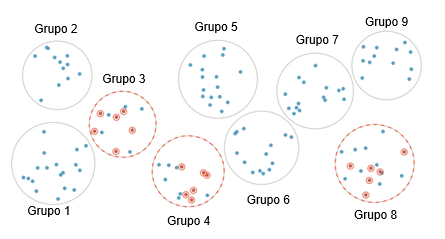
\includegraphics[width=0.9\textwidth]{1-4_obs_studies_sampling/multistage.png}
\end{center}

\end{frame}

%%%%%%%%%%%%%%%%%%%%%%%%%%%%%%%%%%%%

\begin{frame}
\frametitle{Prática}

\pq{
Um conselho municipal solicitou que uma pesquisa domiciliar fosse conduzida em uma área da cidade. A área é dividida em muitos bairros distintos, alguns incluindo grandes casas, alguns apenas com  apartamentos. Qual abordagem seria, provavelmente, \emph{menos} efetiva?}

\begin{enumerate}[(a)]
\item Amostragem aleatória simples
\solnMult{Amostragem por conglomerados}
\item Amostragem Estratificada
\item Amostragem sistemática.
\end{enumerate}

\end{frame}

%%%%%%%%%%%%%%%%%%%%%%%%%%%%%%%%%%%%

